\subsection{Hypercube max line picking}
\label{sec:hypercubemax_line}

\begin{figure}[tbp]
  \begin{center}
    \subfloat[\label{fig:hypercubemax_eg}3-cube max metric example, max distances shown in red.]
       {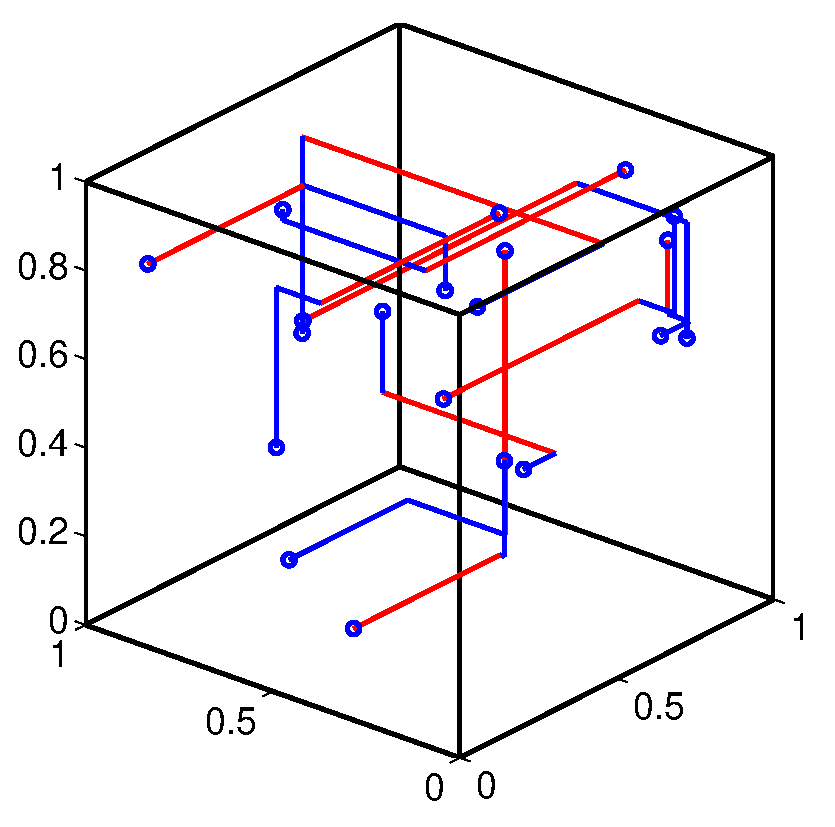
\includegraphics[width=0.4\columnwidth]{../Matlab/Plots/LinePicking_eg_cubemax.eps}} 
    \hspace{6mm}
    \subfloat[\label{fig:hypercubemax_pdf}PDF of $n$-cubes using max metric.]
         {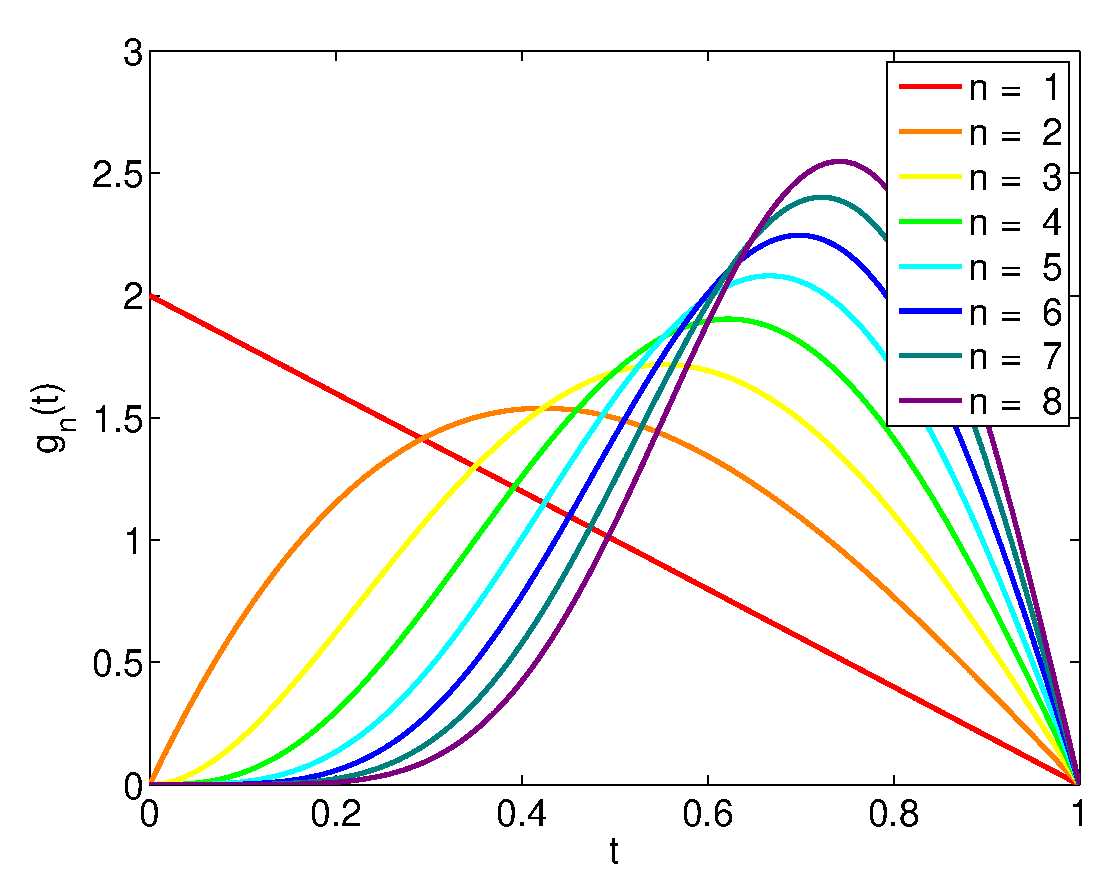
\includegraphics[width=0.48\columnwidth]{../Matlab/Plots/LinePicking_plot_ncubemax.eps}} 
    \caption{The hyperball-line picking problem.}
  \end{center} 
\vspace{-4mm}
\end{figure}

The $n$-Dimensional hyper-cube (or just $n$-cube) with the {\em max} metric is particularly tractable.
Lower order examples are:
\begin{itemize}

\item A 1-cube is a line segment;

\item A 2-cube is a square;

\item A 3-cube is an ordinary cube.


\subsubsection{CDF}

We start by noting that the region is simply the cartesian product of $n$ lines and use the CDF method:

\begin{eqnarray}
 G^{n-{\rm cube max}}_L\left(t\right) & = & \int_{0}^{t} \ldots \int_{0}^{t}   g^{\rm line}_L\left(s_{1}\right)\ldots g^{\rm line}_L\left(s_{n}\right) \;ds_{1}\ldots ds_{n}, \nonumber \\
 & = & \int_{0}^{t}  g^{\rm line}_L\left(s_{1}\right) \;ds_{1}   \ldots \int_{0}^{t} g^{\rm line}_L\left(s_{n}\right) \;ds_{n},\nonumber \\
 & = & \left[\int_{0}^{t}  g^{\rm line}_L\left(s\right) \;ds \right]^{n},\nonumber \\
 & = & \left[G^{\rm line}_L\left(t\right)\right]^{n} ,\nonumber \\
 & = &  \left[\left(\frac{2}{L}\right)\left( t - \frac{t^2}{2L} \right)\right]^{n}.
\end{eqnarray}

\subsubsection{PDF}
To get the PDF we simply differentiate the PDF with respect to $t$:

\begin{eqnarray}
 g^{n-{\rm cube max}}_L\left(t\right) & = & \frac{d G^{n-{\rm cube max}}_L\left(t\right)}{dt},\nonumber \\
& = &  n\left[\left(\frac{2}{L}\right)\left( t - \frac{t^2}{2L} \right)\right]^{n-1} \left[\left(\frac{2}{L}\right)\left( 1 - \frac{t}{L} \right)\right],\nonumber \\
& = &  n\left(\frac{2}{L}\right)^{n} \left( t - \frac{t^2}{2L} \right)^{n-1}\left( 1 - \frac{t}{L} \right), \nonumber \\
\end{eqnarray} 
 
\subsubsection{Moments}

\begin{eqnarray}
E[ X^{k}_{n} ]  & = & \int_0^L t^k  g^{n-{\rm cube max}}_L\left(t\right) \, dt, \nonumber \\
& = &   n\left(\frac{2}{L}\right)^{n} \left(2L\right)^{k + n -1} \int_0^L \left(\frac{t}{2L}\right)^{k + n -1} \left( 1 - \frac{t}{2L} \right)^{n-1}\left( 1 - \frac{t}{L} \right) \; dt.
\end{eqnarray} 

Let $u = \frac{t}{2L}$ then $t = 2uL$ and $dt = du\; 2L$. Thus:
\begin{eqnarray}
E[ X^{k}_{n} ] & = &   n\left(\frac{2}{L}\right)^{n} \left(2L\right)^{k + n -1} \int_0^{\frac{1}{2}} u^{k + n -1} \left( 1 - u \right)^{n-1}\left( 1 - 2u} \right) \; du \; 2L, \nonumber \\
& = &   n 2^{2n + k} L^{k}\left[ \int_0^{\frac{1}{2}} u^{k + n -1} \left( 1 - u \right)^{n-1} \; du\  - 2\int_0^{\frac{1}{2}} u^{1+ k + n -1} \left( 1 - u \right)^{n-1} \; du\right], \nonumber \\
& = &   n 2^{2n + k} L^{k}\left[\beta\left(\frac{1}{2}; k + n, n\right) - 2\beta\left(\frac{1}{2}; k + n + 1, n\right)\right].  
\end{eqnarray}

Means are the first moment and using $\sigma^2 = E[X^2] - E[X]^2$  we can calculate the  variance of these $n$-cubes:
\begin{eqnarray}
 \mu^{\rm 1-cube max}  & = & \frac{L}{3} \nonumber\\
 \mu^{\rm 2-cube max}  & = & \frac{7L}{15} \nonumber\\
 \mu^{\rm 3-cube max }  & = &  \frac{19 L}{35}\nonumber\\
 \mu^{\rm 4-cube max }  & = & \frac{187 L}{315}\nonumber\\
 \mu^{\rm 5-cube max}  & = &  \frac{437 L}{693}\nonumber\\
 \mu^{\rm 6-cube max}  & = & \frac{1979 L}{3003} \nonumber\\
 \mu^{\rm 7-cube max}  & = &  \frac{4387 L}{6435}\nonumber\\
 \mu^{\rm 8-cube max}  & = & \frac{76627 L}{109395}\nonumber\\
 \mu^{\rm 9-cube max}  & = & \frac{165409 L}{230945}\nonumber\\
 \mu^{\rm 10-cube max} & = & \frac{707825 L}{969969}\nonumber 
\end{eqnarray}

\begin{eqnarray}
 \sigma^2_{\rm 1-cube max}  & = & \frac{L^2}{18}\nonumber\\
 \sigma^2_{\rm 2-cube max}  & = & \frac{11L^2}{225} \nonumber\\
 \sigma^2_{\rm 3-cube max }  & = &  \frac{201L^2}{4900}\nonumber\\
 \sigma^2_{\rm 4-cube max }  & = & \frac{3461 L^2}{99225}\nonumber\\
 \sigma^2_{\rm 5-cube max}  & = &  \frac{29011 L^2}{960498}\nonumber\\
 \sigma^2_{\rm 6-cube max}  & = & \frac{239711 L^2}{9018009} \nonumber\\
 \sigma^2_{\rm 7-cube max}  & = &  \frac{7854793 L^2}{331273800}\nonumber\\
 \sigma^2_{\rm 8-cube max}  & = & \frac{255954401 L^2}{11967266025}\nonumber\\
 \sigma^2_{\rm 9-cube max}  & = & \frac{2077184013 L^2}{106671186050}\nonumber\\
 \sigma^2_{\rm 10-cube max} & = & \frac{16811419715 L^2}{940839860961} \nonumber
\end{eqnarray}

